%\documentclass[german,bachelor]{swsLeipzig}
\documentclass[german,bachelor]{swsLeipzig}
% When you change the language, pdflatex may halt on recompilation.
% Just hit enter to continue and recompile again. This should fix it.

%
% Values
% ------
\ThesisSetTitle{Ermittlung von Konfigurationsoptionen im Source Code mit Fokus auf Machine Learning Bibliotheken in Python}
\ThesisSetKeywords{These, Are, My keywords} % only for PDF meta attributes

\ThesisSetAuthor{Marco Jaeger-Kufel}
\ThesisSetStudentNumber{3731679}
\ThesisSetDateOfBirth{10}{05}{1995}
\ThesisSetPlaceOfBirth{Hannover}

\ThesisSetSupervisors{Prof.\ Dr.\ Norbert Siegmund,Prof.\ Dr.\ Unknown Yet}

\ThesisSetSubmissionDate{14}{06}{2022}

%
% Suggested Packages
% ------------------
\usepackage[sort&compress]{natbib}
%   Allows citing in different ways (e.g., only the authors if you use the
%   citation again within a short time).
%
\usepackage{booktabs}
%    For tables ``looking the right way''.
%
%\usepackage{tabularx}
%    Enables tables with columns that automatically fill the page width.
%
%\usepackage[ruled,algochapter]{algorithm2e}
%    A package for pseudo code algorithms.
%
%\usepackage{amsmath}
%    For tabular-style formatting of mathematical environments.
%

%
% Commenting (by your supervisor)
% -------------------------------
\usepackage{xcolor}
\usepackage{soul}
\usepackage{listings}
\usepackage{multirow}
\usepackage[euler]{textgreek}
\usepackage{graphicx}
\usepackage{lscape}
\usepackage{makecell}
\newcommand{\bscom}[2]{%
  % #1 Original text.
  % #2 Replacement text.
    \st{\scriptsize\,#1}{\color{blue}\scriptsize\,#2}%
  }

% Create links in the pdf document
% Hyperref has some incompatibilities with other packages
% Some other packages must be loaded before, some after hyperref
% Additional options to the hyperref package can be provided in the braces []
\usehyperref[backref] % This will add back references in the bibliography
\usepackage[utf8]{inputenc}
\usepackage{textcomp}
\usepackage{tikz,pgfplots}
\usetikzlibrary{shapes.geometric, arrows}
\usetikzlibrary{patterns}
\usepackage{float}
%\setcitestyle{authoryear,close={)}}
%\setcitestyle{author}

\begin{document}
\begin{frontmatter}
  \begin{abstract}
    A short summary.
  \end{abstract}

  \tableofcontents

  %\chapter*{Acknowledgements} % optional
  %I thank the authors of the swsLeipzig template for their excellent work!

  \listoffigures % optional

  \listoftables % optional

  %\listofalgorithms % optional
  %    requires package algorithm2e

  % optional: list of symbols/notation (e.g., using the nomencl package)
\end{frontmatter}

\chapter{Einleitung}\label{Einleitung}
%Diese Arbeit entsteht am Institut für Informatik an der Universit\"at Leipzig in der Abteilung \glqq Softwaresysteme\grqq.
%Im Folgenden wird die zugrundeliegende Problemstellung und Relevanz erl\"autert.
%Anschlie\ss end wird dieses Problem auf einen konkreten Anwendungsbereich \"ubertragen und auf die Zielsetzung der Arbeit eingegangen.\\

\section{Motivation}
Moderne Softwaresysteme erm\"oglichen den Nutzenden ein breites Spektrum unterschiedlicher Konfigurationsoptionen.
Anhand dieser Konfigurationsoptionen sind die Nutzenden in der Lage, viele Aspekte der Ausgestaltung einer Software zu steuern.
Konfigurationsoptionen k\"onnen dabei ganz unterschiedliche Funktionen besitzen, die von den Nutzenden nach den eigenen Bed\"urfnissen angepasst werden k\"onnen.\\

Konfigurationsoptionen können in verschiedenen Teilen eines Softwareprojekts verarbeitet, definiert und beschrieben werden,
wie beispielsweise in der Konfigurationsdatei, im Source Code und in der Dokumentation \cite[]{7774519}.
Sie werden meist als Key-Value Pair entworfen und gesammelt in einer Konfigurationsdatei gespeichert.
Dem Namen der Konfigurationsoption (Key) werden dabei Einstellungsmöglichkeiten beliebigen Typs zugeordnet (Value).
Zur Speicherung von Konfigurationsoptionen verwenden einige Systeme, wie das Big Data-Framework Hadoop, strukturierte XML-Formate oder auch JSON-Dateien.
Ein einheitliches Schema zur Speicherung als Konfigurationsdatei gibt es jedoch nicht, weshalb sich diese von der Struktur und Syntax unterscheiden \cite[]{10.1145/1985793.1985812}.
Im Source Code können die Konfigurationsoptionen eingelesen und bearbeitet werden \cite[]{7774519}.\\

W\"ahrend die Vielf\"altigkeit und Individualisierbarkeit der Software gr\"o\ss er wird, erh\"oht sich auch die Komplexit\"at der Software f\"ur Entwickler und Entwicklerinnen.
Vor allem das Warten und Testen der Konfigurationsmöglichkeiten gestaltet sich nun umfangreicher.
Besonders problematisch wird es, wenn Konfigurationsoptionen auf unvorhergesehene Weise interagieren.
Solche Abh\"angigkeiten sind in einem wachsenden Spielraum m\"oglicher Kombinationen schwer zu entdecken und zu verstehen.
Entwickler und Entwicklerinnen m\"ussen die Konfigurationsoptionen innerhalb der Software verfolgen, um festzustellen,
welche Codefragmente von einer Option betroffen sind und wo und wie sie mit ihr interagieren.
Des Weiteren kann es vorkommen, dass Entwickler und Entwicklerinnen Werte von Konfigurationsoptionen nicht aktualisieren, was dazu führen kann,
dass über mehrere Module hinweg, unbemerkt mit falschen Werten gearbeitet wird \cite[]{7774519}.
Die verschiedenen m\"oglichen Auspr\"agungen einer Konfigurationsoption erschweren hierbei die Nachvollziehbarkeit des Kontrollflusses der Software.\\

In einer empirischen Studie über Konfigurationsfehler stellen \citeauthor{10.1145/2043556.2043572} fest,
dass in kommerziellen Softwareunternehmen für Speicherlösungen, knapp ein Drittel aller Ursachen von Kundenproblemen auf Konfigurationsfehler zurückzuführen sind (siehe Tabelle 3).
Bei Konfigurationsfehler sind Source Code und die Eingabe zwar korrekt, es wird jedoch ein falscher Wert für eine Konfigurationsoption verwendet,
sodass sich die Software nicht wie gewünscht verhält.
Solche Fehler können dazu führen, dass die Software abstürzt, eine fehlerhafte Ausgabe erzeugt oder nur unzureichend funktioniert \cite[]{10.1145/2568225.2568251}.\\

Konfigurationsfehler entstehen zum Beispiel durch die Verwendung unterschiedlicher Versionen einer Software.
Im folgendem Codeausschnitt wird die Klasse \textit{LogisticRegression} der Machine Learning-Bibliothek \textit{scikit-learn} initialisiert und der Variable \textit{clf} zugewiesen:\\

\begin{lstlisting}[language=Python, frame=single, basicstyle=\small]
from sklearn.linear_model import LogisticRegression
clf = LogisticRegression()
\end{lstlisting}
\

Da keine Parameter angegeben werden, wird die Klasse mit den Default-Werten initialisiert, zum Beispiel
\textit{max\_iter = 100, verbose = 0, n\_jobs = 1}.
In der Version \textit{scikit-learn 0.21.3} wird für den Parameter \textit{multi\_class} als Default noch der Wert \textit{ovr} zugewiesen (\citeyear{sklearn}).
Für alle nachfolgenden Versionen ist der Default-Wert für diesen Parameter jedoch \textit{auto} (\citeyear{sklearn}).
Folglich führt die Verwendung dieser Klasse ohne explizite Parameterangabe, nach Verwendung unterschiedlicher Versionen, zu schwer nachvollziehbaren Programmverhalten.\\

Bei den Parametern eines solchen Machine Learning Algorithmus, die vor Beginn des Lernprozesses vom Nutzenden festgelegt werden können,
spricht man dabei von sogenannten \textit{Hyperparametern}.
Sie werden als Parameter an die jeweilige Klasse übergeben und bieten den Nutzenden Konfigurationsmöglichkeiten für
das Training des Modells.
In dem obigen Fall können so beispielsweise über den Parameter \textit{max\_iter} die Anzahl der Trainingsiterationen
der Logistischen Regression festgelegt werden und über \textit{n\_jobs} die maximale Anzahl der parallel zu verwendenden CPU-Kernen.
Durch das Extrahieren dieser Konfigurationswerte, können die Parameter statisch geprüft werden, was für den Nutzenden
eine Zeitersparnis bedeutet, wenn sonst ein falscher Konfigurationswert einen langen Batch-Job zum Scheitern bringt
oder das Ergebnis nicht den Erwartungen entspricht. \\



\section{Zielsetzung}
Das Ziel dieser Arbeit ist es, Konfigurationsoptionen im Source Code zu erkennen und zu extrahieren. \\

Es existieren bereits einige Forschungsansätze zur Ermittlung und Verarbeitung von Konfigurationsoptionen im Source Code.
Viel zitiert wird dabei der Ansatz von \citeauthor{10.1145/1985793.1985812}, den sie \citeyear{10.1145/1985793.1985812} publizierten.
Wie auch \citeauthor{7774519} oder \citeauthor{8049300} entwickelten sie einen Ansatz, mittels statischer Code-Analyse Konfigurationsoptionen
im Source Code zu tracken.
Dabei fokussierten sie sich auf die Programmiersprache Java, die nach dem TIOBE-Index jahrelang als beliebteste Programmiersprache galt.
Der TIOBE-Index misst die Popularität von Programmiersprachen auf der Grundlage von Suchanfragen auf beliebten Websites und in Suchmaschinen.
Im Februar 2022 ist in diesem Ranking Python erstmals zur beliebtesten Programmiersprache aufgestiegen \cite[]{enwiki:1077809155}.
Für Python ist diese Thematik jedoch bislang allerdings noch wenig beleuchtet. \\

Die Programmiersprache Python ist für ihre Benutzendenfreundlichkeit bekannt und obwohl Python eine interpretierte High-Level-Programmiersprache ist,
ist sie in der Lage, bei Bedarf die Leistung von Programmiersprachen auf Systemebene zu nutzen.
Insbesondere im Bereich wissenschaftliches Rechnen (Scientific Computing) gewann Python in den letzten Jahren enorm an Popularität,
weshalb viele Bibliotheken für maschinelles Lernen auf Python basieren \cite[]{2020}.\\

Gegenstand dieser Arbeit werden daher Konfigurationsoptionen von ML Algorithmen in Python Source Code, die mittels statischer Code-Analyse erkannt werden.
Der Ansatz identifiziert automatisch die Stellen im Source Code, an denen die Optionen der zu untersuchenden Bibliotheken gelesen werden
und ermittelt für jede dieser Stellen den Namen der Option.
Darauf aufbauend erfolgt eine Datenflussanalyse, um auch für Optionen, die in Form von Variablen als Parameter übergeben werden,
die möglichen Werte zu ermitteln.
Der Fokus liegt auf drei der populärsten Machine Learning Bibliotheken in Python (siehe \autoref{fig:kaggle}):
\begin{itemize}
 \item TensorFlow
 \item PyTorch
 \item scikit-learn
\end{itemize}
Zudem wird die Verwendung von Konfigurationsoptionen der Machine Learning Lifecylce Plattform \textit{MLflow} untersucht. \\


\section{Aufbau dieser Arbeit und methodisches Vorgehen}
% Umsetzung gleidert isch in 3 Schritte: WEbscrping, nochmal auf Klassen eingehen, Statische Code-Analyse mit ReadPoint, und extrahieren der Parameter,
% Am Ende einfpelgen in s Cg net

\chapter{Hintergrund}\label{Hintergrund}

\section{Statische Code-Analyse}
Das wichtigste Werkzeug dieser Arbeit ist die statische Code-Analyse,
mit der Software-Projekte unabhängig von der Ausführungsumgebung untersucht werden können.
Die statische Code-Analyse ist ein Werkzeug, um Fehler in einer Softwareanwendung zu reduzieren.
So ermöglichen sie den Anwendenden, Fehler in einem Programm zu finden, die für den Compiler nicht sichtbar sind \cite[]{bardas2010static}.\\

Im Gegensatz zur dynamischen Analyse wird die statische Analyse zur Übersetzungszeit durchgeführt
und setzt damit bereits vor der tatsächlichen Ausführung des Source Codes an.
Die erzeugten Ergebnisse der statischen Analyse lassen sich besser Verallgemeinern, da sie nicht abhängig von den Eingaben sind,
mit denen das Programm während der dynamischen Analyse ausgeführt wurde \cite[]{gomes2009overview}.\\

Für das Aufspüren von Konfigurationsoptionen bietet sich eine statische Code-Analyse daher aus mehreren Gründen an.
So kann es viele Optionen geben, die nur in bestimmten Modulen oder als Folge bestimmter Eingaben verwendet werden.
%Es ist unwahrscheinlich, dass mittels dynamischen Testens alle Verwendungen der gesuchten Konfigurationsoptionen gefunden werden.
%Dies würde zudem bei größeren Softwareprojekten eine sehr komplexe Test-Suite erfordern, um möglichst alle Fälle abdecken zu können.
Mit der statischen Code-Analyse kann eine hohe Abdeckung hingegen deutlich leichter erreicht werden.
Gleichzeitig verbergen sich hinter den Methoden und Klassen, der zu untersuchenden Machine Learning Bibliotheken,
teils sehr komplexe und rechenintensive Berechnungen, die bis zu mehreren Tagen laufen könnten.
Aus Kosten-Nutzen-Gründen ist hier eine dynamische Analyse nur bedingt sinnvoll.\\

\section{Datenflussanalyse}
Die Datenflussanalyse ist ein Werkzeug, um Informationen über die möglichen Werte, die an verschiedenen
Stellen in einem Codesegment berechnet werden, zu erfassen \cite[]{58766}.
Es handelt sich um eine statische Analysetechnik mit dem Ziel, das Programmverhalten schon zur Übersetzungszeit,
also bevor es ausgeführt wurde, zu bestimmen.
Der Datenfluss kann mittels eines Kontrollflussgraphens dargestellt werden und dem Betrachtenden
Rückschlüsse über das Verhalten des Programms geben.
Der Graph zeigt an, an welchen Stellen eine Variable verwendet wird und welche Werte sie annehmen kann.\\

Es gibt verschiedene Techniken, die innerhalb der Datenflussanalyse eingesetzt werden, um den Wert von Variablen zu bestimmen.
Eine von ihnen ist \textit{Constant Propagation}.
Das Ziel von Constant Propagation ist zu bestimmen, an welchen Stellen im Programm, eine Variable einen konstanten Wert besitzt.
So kann zum Beispiel toter Code, also redundanter Code, der im weiteren Programmverlauf nicht weiterverarbeitet wird, gefunden werden.\\

Eine weitere Technik ist \textit{Static Single Assignment}.
Bei dieser Methodik werden die Variablen im Verlauf des Übersetzungsprozesses in eine Zwischenform überführt, in der jede Variable
genau einmal zugewiesen wird.
Die Variablen werden in Versionen aufgeteilt und in der Regel mit einem aufsteigendem Index versehen,
sodass jede Definition ihre eigene Version erhält.\\

Die beide Techniken Static Single Assignment und Constant Propagation werden in dem statischen Analyse-Framework
\textit{Scalpel} kombiniert.
Aus dem folgenden Codebeispiel geht hervor, dass die Variable \textit{a} zwei unterschiedliche Werte annehmen kann.\\

\begin{lstlisting}[language=Python, frame=single, basicstyle=\small]
c = 10
a = -1
if c > 0:
    a = a + 1
else:
    a = 0
total = c + a
\end{lstlisting}
\

Der daraus resultierende Kontrollflussgraph besteht charakteristisch aus Knoten, die die jeweilige Code-Objekte beinhalten und gerichtete Kanten als Übergang
zwischen den Knoten, die den Programmablauf darstellen.
Mittels Constant Propagation werden die tatsächlichen Werte der Variablen an den jeweiligen Verwendungszeitpunkten erkannt
und über die \textPhi-Funktion kann durch Static Single Assignment abgeleitet werden, dass es zwei mögliche Rückgabewerte gibt.

\begin{figure}[h]
 \centering
 \includegraphics[scale=0.8]{ssa_diagram}
 \caption{Kontrollflussgraph \cite[]{li2022scalpel}}
 \label{fig:scalpel}
\end{figure}


\section{Maschinelles Lernen}
Die künstliche Intelligenz (KI) ist ein Teilgebiet der Informatik und befasst sich mit der Entwicklung von Computerprogrammen und Maschinen,
die in der Lage sind, Aufgaben auszuführen, die Menschen von Natur aus gut beherrschen.
Dazu gehören zum Beispiel die Verarbeitung von natürlicher Sprache (Natural Language Processing) oder Bilderkennung (Computer Vision).
In der Mitte des 20. Jahrhunderts entstand das maschinelle Lernen (ML) als Teilbereich der KI und schlug eine neue Richtung
für die Entwicklung von künstlicher Intelligenz ein, inspiriert vom konzeptionellen Verständnis der Funktionsweise des menschlichen Gehirns \cite[]{2020}.\\

Pionier Arthur Samuel definiert maschinelles Lernen als ein Fachgebiet, das Computern die Fähigkeit verleiht, zu lernen,
ohne ausdrücklich programmiert zu werden.
Es befasst sich mit der wissenschaftlichen Untersuchung von Algorithmen und statistischen Modellen,
die Computersysteme verwenden, um eine Aufgabe zu lösen \cite[]{mahesh2020machine}.
Dabei werden statistische Methoden verwendet, um aus Daten zu lernen und Muster zu erkennen. \\




%Maschinelles Lernen (ML) wird eingesetzt, um Maschinen beizubringen, wie sie Daten effizienter verarbeiten können.
%Manchmal können wir nach der Sichtung der Daten die Informationen, die wir aus den Daten gewinnen, nicht interpretieren.
%In diesem Fall wenden wir maschinelles Lernen an.
%Mit der Fülle der verfügbaren Datensätze steigt auch die Nachfrage nach maschinellem Lernen.
%Viele Branchen setzen maschinelles Lernen ein, um relevante Daten zu extrahieren.
%Der Zweck des maschinellen Lernens besteht darin, aus den Daten zu lernen.
%Es wurden viele Studien darüber durchgeführt, wie Maschinen selbständig lernen können, ohne explizit programmiert zu werden.
%Viele Mathematiker und Programmierer wenden verschiedene Ansätze an, um eine Lösung für dieses Problem zu finden, das riesige Datensätze umfasst.

%\subsection{Ursprung}
%Der Ursprung des maschinellen Lernens liegt bereits in der Mitte des 20. Jahrhunderts, als der Psychologoe Frank Rosenblatt
%von seiner Arbeitsgruppe eine Maschine zur Erkennung von Buchstaben des Alphabets bauen ließ \cite[S. 1385]{FRADKOV20201385}.
%Das Konzept der Maschine basiert auf der Verarbeitung von Signalen analog zum menschliche Nervensystem, weshalb sie
%als Prototyp der modernen künstlichen neuronalen Netze gilt \cite[S. 1385]{FRADKOV20201385}.
%Der kommerzielle Durchbruch ließ dennoch bis auf den Anfang des 21. Jahrhunderts auf sich warten.
%Nach \citeauthor{FRADKOV20201385} ist dies auf drei Trends zurückzuführen, die zusammen einen spürbaren Synergieeffekt bewirkten \cite[S. 1387]{FRADKOV20201385}. \\

%Unter anderem durch den Erfolg und Möglichkeiten des Internets ist nicht nur das Vorhandensein von Daten enorm gewachsen,
%auch ihre Heterogenität führt dazu, dass herkömmliche Methode zur Verarbeitung und Informationsgewinnung nicht mehr ausreichen \cite[S. 1387]{FRADKOV20201385}.
%Durch das Aufkommen von \textit{Big Data} werden neue Ansätze des maschinellen Lernens nicht nur aus dem Motiv des wissenschaftlichen Erkenntnisgewinns entwickelt,
%sondern auch aufgrund der praktischen und kommerziellen Notwendigkeit, die rasant wachsenden generierten Datenmengen leistungsfähig verarbeiten zu können. \\

%Ein weiterer entscheidender Faktor ist die Senkung der Kosten für parallele Berechnung und Speicher.
%Dies umfasst die Weiterentwicklung und Verwendung von Grafikprozessoren (vor allem von Nvidia),
%die zu erheblichen Verbesserungen der Rechenleistung führen \cite[S. 1387]{FRADKOV20201385}.
%Gleichzeitig sinken die Kosten für Arbeitsspeicher stetig, was die Verarbeitung großer Datenmengen zusätzlich erleichtert \cite[S. 1387]{FRADKOV20201385}.
%Aus Softwaresicht kommt schließlich die MapReduce-Technologie von Google bzw. später auch Hadoop hinzu, die es ermöglicht,
%komplexe Berechnungen auf mehrere Prozessoren zu verteilen\cite[S. 1387]{FRADKOV20201385}. \\

%Der dritte Trend ist die Entwicklung künstlicher neuronaler Netze, die um ein Vielzahl an Zwischenschichten erweitert wurden
%und so noch komplexere Berechnungen ausführen können.
%In diesem Zusammenhang spricht man auch von \textit{Deep Learning}. \\

%\subsection{Algorithmische Ansätze}
%Im Allgemeinen werden die Ansätze des maschinellen Lernens in drei große Kategorien unterteilt, je nach Art des \textit{Signals}
%oder \textit{Feedbacks}, das dem lernenden System zur Verfügung steht \cite[S. 2]{FRADKOV20201385}:
%\begin{itemize}
% \item Überwachtes Lernen (supervised learning)
% \item Unüberwachtes Lernen (unsupervised learning)
% \item Bestärkendes Lernen (reinforcement learning)
%\end{itemize}

%Das \textit{überwachte Lernen} erfordert ein Training mit gelabelten Daten, die Eingaben und gewünschte Ausgaben haben \cite[S. 2]{cite-key}.
%So weiß das Modell zum Beispiel, ob auf einem bestimmten Foto ein Hund abgebildet ist oder wie viel ein bestimmtes Haus kostet.
%Auf dieser Grundlage kann es dann so trainiert werden, dass es neue Hunde erkennt oder den Preis neuer Häuser schätzt. \\

%Im Gegensatz dazu erfordert das \textit{unüberwachte Lernen} keine markierten Trainingsdaten und erhält lediglich Eingabedaten \cite[S. 2]{cite-key}.
%Die richtige Antwort ist entweder nicht bekannt oder existiert nicht.
%Stattdessen sucht das Modell nach sinnvollen Strukturen in den Daten, um neue Erkenntnisse über ein Thema zu gewinnen \cite[S. 383]{mahesh2020machine}.
%Unüberwachtes Lernen kann zum Beispiel dazu verwendet werden, in einem Online-Store Kunden zu finden, die einen ähnlichen Geschmack haben,
%und Artikel empfehlen, die diese Kunden gekauft haben. \\

%Das \textit{bestärkende Lernen} hingegen unterscheidet sich sehr deutlich von den beiden vorherigen Kategorien.
%Das Modell ist hier ein aktiver Akteur, das mit seiner externen Umgebung interagiert
%und positives oder negatives Feedback für seine Handlungen erhält \cite[S. 2]{cite-key}.
%Aus diesen Rückmeldungen erlernt es optimale Handlungsstrategien für seine Umgebung zu entwickeln \cite[S. 384]{mahesh2020machine}.
%Solche Modelle können zum Beispiel für selbstfahrende Autos verwendet werden oder um einer Maschine Gesellschaftsspiele beizubringen.\\

\subsection{Python-Bibliotheken}
Fürs maschinelle Lernen gilt Python schon seit langem als erste Wahl für Entwickler und Entwicklerinnen.
Eine im Mai \citeyear{nugget} veröffentlichte Umfrage vom Portal \citeauthor{nugget} ergab, dass Python in der Kategorie
\glqq Top Analytics, Data Science, Machine Learning Tools\grqq{} von rund 66\% der Teilnehmenden verwendet wird
und damit die populärste Programmiersprache in diesem Bereich ist \cite[]{nugget}. \\

Python ist eine interpretierte Programmiersprache.
Demnach wird während der Ausführung der Python-Code zur Laufzeit interpretiert, wodurch sie im Vergleich mit kompilierten
Programmiersprachen wie C / C++ hinsichtlich Leistung und Geschwindigkeit schlechter abschneidet.
Ein wichtiger Vorteil von Python ist jedoch die Möglichkeit, Code aus anderen Programmiersprachen relativ einfach einzubinden.
Viele Lösungen im maschinellen Lernen basieren auf numerischen und vektorisierten Berechnungen mit Bibliotheken
wie \textit{NumPy} oder \textit{SciPy}.
Um diese Berechnungen schnell und effizient auszuführen, werden sogenannte \textit{Wrapper} verwendet,
die Algorithmen von kompilierten Programmiersprachen implementieren.
Die wahrscheinlich am häufigsten verwendete Bibliothek für diesen Zweck ist Cython, die zwar auf Python basiert,
aber auch den Aufruf von Funktionen, sowie die Verwendung von Variablen und Klassen aus der Programmiersprache C unterstützt \cite[]{8757088}.
Dadurch können kritische Teile des Codes um ein Vielfaches beschleunigt werden. \\

Einer der Hauptgründe für die Popularität von Python ist das riesige Ökosystem, das aus einer Vielzahl
von umfangreichen und leistungsfähigen Bibliotheken besteht, über die ML-Algorithmen aufgerufen werden können,
wodurch die Benutzendenfreundlichkeit bei gleichzeitiger Effizienz in der Performanz gewahrt bleiben kann \cite[]{2020}.
So sind nach einer jährlich von der Data Science-Plattform \citeauthor{kaggle} durchgeführten Umfrage unter rund 25.000 ML-Engineers
und Data Scientists, die Python Bibliotheken mit großem Abstand die am meisten genutzten Frameworks für maschinelles Lernen \cite[]{kaggle}.\\

Eine Python-Bibliothek entspricht einer Sammlung zusammenhöriger Module, die aus vorkompiliertem Code bestehen.
Nach erfolgreicher Installation werden die Funktionalitäten der jeweiligen Bibliothek über die \textit{import}-Anweisung für ein Programm zugänglich
gemacht.
Entwickler und Entwicklerinnen können nun die vorprogrammierten Klassen und Methoden aufrufen und beliebig verwenden,
ohne die hinterlegten Algorithmen kennen zu müssen.

\subsection{ML Konfigurationsoptionen} \label{ML Konfigurationsoptionen}
In objektorientierten Programmiersprachen wie Python sind Klassen einer der grundlegenden Bausteine, die bei der Entwicklung und Anwendung
von maschinellem Lernen eingesetzt werden.
Sie bieten die Möglichkeit, Daten und Funktionen zu kombinieren und dem Nutzenden von Machine Learning Bibliotheken,
bereits vorformulierte Algorithmen aufzurufen.
Dabei werden die Konfigurationsoptionen beim Aufruf der jeweiligen Klasse als Parameter übergeben, sodass die Algorithmen
an die Bedürfnisse des Anwendenden angepasst werden können.
So kann die zielgerichtete Nutzung effizienter und komplexer Algorithmen bei gleichzeitiger Konfigurierbarkeit gewährleistet werden. \\

Bei den Konfigurationsparametern von Lernalgorithmen handelt es sich um sogenannte \textit{Hyperparameter}.
Lernalgorithmen ermöglichen einem Computerprogramm, den menschlichen Lernprozess mittels statistischer Methoden zu imitieren.
Sie werden zur Mustererkennung, Klassifizierung und Vorhersage verwendet, indem sie aus einem vorhandenen Trainingsdatensatz
lernen.
Hyperparameter werden festgelegt bevor der Lernprozess beginnt und um den Lernprozess zu steuern \cite[]{hype}.
Da sich die Algorithmen oft sehr unterschiedlich verhalten, wenn sie mit verschiedenen Hyperparameter instanziiert werden,
wurden in den letzten Jahren eine Vielzahl an Hyperparameter-Optimierungsverfahren entwickelt \cite[]{pmlr-v32-hutter14}.
Optimierte Hyperparameter können die Leistungsfähigkeit eines Modells oder die Geschwindigkeit und Qualität Lernprozesses stark beeinflussen \cite[]{hype}.\\

Im folgenden Codebeispiel wird der \textit{Gradient Boosting Classifier} aus der scikit-learn Bibliothek betrachtet.\\

\begin{lstlisting}[language=Python, frame=single, basicstyle=\small]
from sklearn.ensemble import GradientBoostingClassifier

gbc = GradientBoostingClassifier(n_estimators=20,
        learning_rate=0.05, max_features=2, max_depth=2,
        random_state=0)
\end{lstlisting}
\

Es wird eine Instanz dieser Klasse erzeugt und der Variable \textit{gbc} zugewiesen.
Die Klasse verfügt über 20 Parameter (Version 1.0.2), die, sofern bei der Instanziierung für den jeweiligen Parameter
kein neuer Wert zugewiesen wird, mit einem eigenen Default-Wert initialisiert werden.
So werden im Beispiel, den Hyperparametern wie \textit{n\_estimators}, \textit{learning\_rate} oder \textit{max\_depth}
Zahlenwerte übergeben, die von den Default-Werten abweichen.\\


\section{Web Scraping}
Web Scraping ist eine Technik, um Daten aus dem World Wide Web zu extrahieren, um sie später abrufen oder analysieren zu können.
Dafür werden die Webdaten über das Hypertext Transfer Protocol (HTTP) oder über einen Webbrowser ausgelesen.
Dies kann entweder manuell durch den jeweiligen Benutzenden oder automatisch durch einen Bot oder Webcrawler erfolgen \cite[]{zhao2017web}.
Ein Web Scraper simuliert das menschliche Browsing-Verhalten im Web, um aus verschiedenen Websites
detaillierte Informationen in einer vorgegebenen Struktur zu sammeln.
Durch die Möglichkeit, für eine bestimmte Website-Struktur systematisch ausgerichtet und programmiert zu werden, liegt der Vorteil
eines Web Scrapers in seiner Automatisierungsfähigkeit und Geschwindigkeit \cite[]{9005594}.
Mögliche Anwendungsfälle sind zum Beispiel das Überwachen von Preis-Änderungen in Online-Shops oder das Auslesen und Kopieren
von Kontaktinformationen.\\

Ein Web Scraping-Prozess gliedert sich üblicherweise in zwei Schritten \cite[]{zhao2017web}:
\begin{enumerate}
 \item Erfassen der Webressourcen
 \item Extrahieren der gewünschten Informationen aus den erfassten Daten
\end{enumerate}
Zunächst wird die Kommunikation zur Ziel-Website über das HTTP-Protokoll hergestellt \cite[]{10.1093/bib/bbt026}.
Über die HTTP-Anfrage ist der Scraper in der Lage, die Ressourcen der jeweiligen Website zu erfassen \cite[]{zhao2017web}.
Dies erfolgt entweder als URL mit einer GET-Abfrage für Ressourcenanfragen oder als HTTP-Nachricht mit einer
POST-Abfrage für die Übermittlung von Formularen \cite[]{10.1093/bib/bbt026}.
Nachdem die Anfrage erfolgreich empfangen und von der Ziel-Website verarbeitet wurde, wird die angeforderte Ressource
von der Website aufgerufen und an das Web Scraping-Programm zurückgesendet.
Die Ressource kann in verschiedenen Formaten vorliegen:
In Auszeichnungssprachen wie HTML (Hypertext Markup Language) oder XML (Extensible Markup Language), JSON-Format
(JavaScript Object Notation) oder in Form von Multimedia-Daten wie Bilder-, Audio oder Videodateien \cite[]{zhao2017web}.\\

Im zweiten Schritt folgt der Extraktionsprozess.
Die heruntergeladenen Daten können nun geparst werden, um die benötigten Informationen zu filtern und in ein geeignetes Format
umzuwandeln \cite[]{10.1093/bib/bbt026}.
Die Daten können nun weiterverarbeitet werden, indem sie beispielsweise analysiert oder in eine gewünschte Struktur
organisiert werden.\\


\section{Abstract Syntax Trees}
Um die Bedeutung von Abstract Syntax Trees (AST) zu verstehen, ist es hilfreich sich zu vergegenwärtigen, welche Prozesse
bei der Ausführung eines Python-Skripts im Hintergrund ablaufen.
Als eine interpretierte High-Level-Programmiersprache wird der Source Code in Python nicht kompiliert, sondern vom
Python Interpreter nach einer bestimmten Abfolge von Schritten in Anweisungen übersetzt.
Dabei wird der Python Code in Bytecode umgewandelt, sodass dieser von der Python Virtual Machine
übersetzt und ausgeführt werden kann. \\

Zunächst wird der Code geparst und in sogenannte Tokens unterteilt.
Diese Tokens unterliegen einer Reihe von Regeln, damit die verschiedenen Programmierkonstrukte unterschiedlich erkannt
und behandelt werden können.
Die Liste an Tokens werden dann in eine Baumstruktur, den sogenannten abstrakten Syntaxbaum (Abstract Syntax Tree), umgewandelt.
Ein AST ist eine baumartige Darstellung des Codes, bestehend aus einer Sammlung von Knoten, die, basierend auf der Grammatik
in Python, miteinander verbunden sind.
Der Baum wird in maschinenlesbaren Binärcode umgewandelt und Anweisungen in Bytecode an den Python Interpreter übermittelt.
Der Python Interpreter kann den Code nun ausführen und Systemaufrufe an den Kernel starten, um das Programm zu starten. \\

Während Bytecode eher für Maschinen gemacht ist, sind Abstract Syntax Trees strukturiert aufgebaut und auch für den Menschen lesbar.
Im Anhang befindet sich das Codebeispiel aus \ref{Konfigurationsoptionen}, nachdem es als AST geparst wurde.
Aus der AST-Syntax lassen sich Typ und Struktur einzelner Python Komponenten direkt ablesen.
So besteht das Modul aus zwei Codeobjekten vom Typ \textit{ImportFrom} und \textit{Assign}, die sich jeweils in kleinere
Objekte verschiedenen Typs unterteilen lassen.
Diese Datenstruktur stellt alle relevanten Informationen für die Ausführung des Codes bereit.
Jeder Knoten des Baumes kann nun besucht werden, um seine Daten zu verarbeiten und entsprechende Aktionen einzuleiten.
Über das \textit{ast}-Modul in Python kann der Code als AST verarbeitet und visualisiert werden, sodass er von
Entwicklern und Entwicklerinnen entsprechend seiner AST-Syntax analysiert und manipuliert werden kann.\\


\chapter{Verwandte Arbeiten}\label{Verwandte Arbeiten}
Zwar wurden bereits einige Ansätze zum Auffinden von Konfigurationsoptionen publiziert, jedoch ist diese Thematik im Rahmen von
maschinellem Lernen kaum beleuchtet.
Die meisten Ansätze, wie der von \citeauthor{10.1145/1985793.1985812} aus dem Jahre \citeyear{10.1145/1985793.1985812},
behandeln Anwendungen in der Programmiersprache Java und ermitteln Konfigurationsoptionen mittels statischer Code-Analyse.
Der von \citeauthor{10.1145/1985793.1985812} entwickelte \textit{Confalyzer} ist vermutlich einer der ersten bekannteren
Tools, die sich mit der Thematik befassen.
Unter der Annahme, das Konfigurationsoptionen als Key-Value Pair vorliegen, betrachtet der Confalyzer Methoden, die mit
dem für Java typischen Schlüsselwort \textit{get} in der Konfigurationsklasse beginnen.
Mittels eines Aufrufgraphens (Call Graph) identifiziert der Confalyzer, wo die Methoden im Source Code aufgerufen werden.
An den jeweiligen Aufrufstellen kann er dann die Konfigurationsoptionen aus den String-Parametern ablesen.
Der Ansatz beruht auf der Annahme, dass viele Konfigurationsoptionen auf ähnliche Weise verwendet werden und bestimmte
Muster ableitbar sind \cite[]{10.1145/1985793.1985812}.\\

Der von \citeauthor{7774519} entwickelte \textit{ORPLocator} orientiert sich an dem Confalyzer und vergleicht sich mit diesem.
Der ORPLocator untersuchte dieselben Java-Frameworks wie beispielsweise Hadoop und konnte mehr dokumentierte
Optionen und dementsprechend auch mehr Verwendungen im Source Code finden.
Dies liegt unter anderem daran, dass der gesamte Source Code nach Aufrufstellen von Konfigurationsschnittstellen durchsucht wird,
während der Confalyzer einen Aufrufgraphen erstellt, der manche Optionen nicht erfasst \cite[]{7774519}.\\

Einen anderen Ansatz verfolgten \citeauthor{8049300} bei der Entwicklung von \textit{Lotrack}.
Lotrack ist ein Tool, das mittels einer erweiterten Taint-Analyse, einer Datenflussanalyse, die externe Daten
(Eingabedaten) über den gesamten Kontrollfluss verfolgt, eine Konfigurations-Map erstellt.
Die Konfigurations-Map beschreibt, welche Codefragmente von Konfigurationsoptionen abhängen und hilft dabei die
Beziehungen zwischen dem konkreten Programmverhalten und der Konfiguration zu finden.
Der Fokus liegt auf Anwendungen, die auf Android-Systemen laufen \cite[]{8049300}. \\

Weitere Ansätze wie der \textit{PrefFinder} von \citeauthor{10.1145/2642937.2643009} verwenden zusätzlich auch dynamische
Analysetechniken, um Konfigurationsoptionen nicht nur zu extrahieren, sondern auch in einer Datenbank zur Abfrage und
Verwendung zu speichern.
Der \textit{Software Configuration Inconsistency Checker} (SCIC) hingegen von \citeauthor{10.1145/2786805.2786869}
erweitert die Extraktion von Konfigurationsoptionen im Key-Value-Modell des Confalyzer um ein baumstrukturiertes Modell.
Im Gegensatz zu anderen Tools, ist dieses auch in der Lage, mehrere Programmiersprachen zu verarbeiten.
Ziel dieses Tools ist die Identifikation von Konfigurationsfehlern \cite[]{10.1145/2786805.2786869}.\\


\chapter{Methodik}\label{Methodik}


\section{Auswahl der Python-Bibliotheken}
Bevor auf das Vorgehen zur Extraktion von Konfigurationsoptionen genauer eingegangen wird, werden an dieser Stelle die
zu untersuchenden Python-Bibliotheken beschrieben.
Im folgenden Abschnitt werden Repositorys beleuchtet, die diese Bibliotheken importieren und verwenden.\\

\begin{figure}[H]
\begin{center}
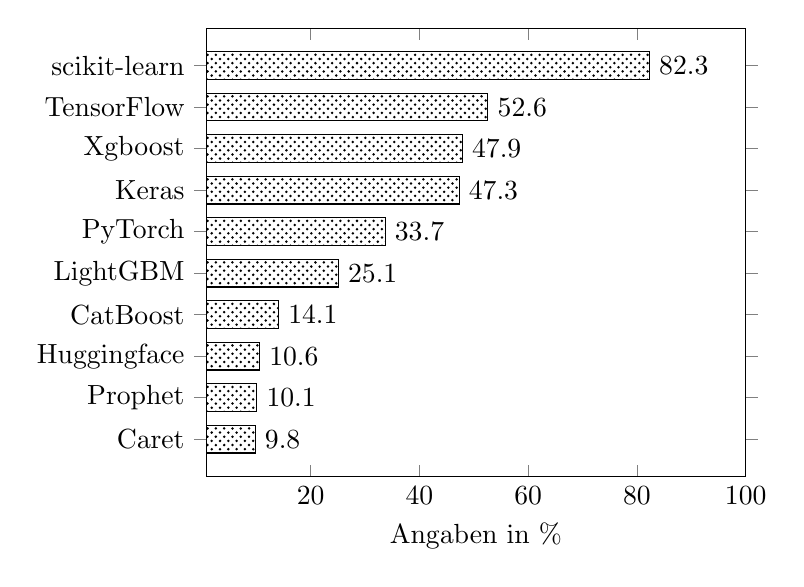
\begin{tikzpicture}
    \begin{axis}[
        xbar,
        xmax=100,
        nodes near coords,
        xlabel={Angaben in \%},
        symbolic y coords={Caret,Prophet,Huggingface,CatBoost,LightGBM,PyTorch,Keras,Xgboost,TensorFlow,scikit-learn},
        ytick = data,
  ]
  \addplot [pattern=crosshatch dots,pattern color=black] coordinates { (82.3,scikit-learn)(52.6,TensorFlow)(47.9,Xgboost)(47.3,Keras)(33.7,PyTorch)(25.1,LightGBM)(14.1,CatBoost)(10.6,Huggingface)(10.1,Prophet)(9.8,Caret)};
  \end{axis}
\end{tikzpicture}
\caption{Nutzung von ML-Frameworks \cite[]{kaggle}} \label{fig:kaggle}
\end{center}
\end{figure}

Aus der Grafik lassen sich drei der zu untersuchenden Python Bibliotheken entnehmen.
Zum einen \textit{scikit-learn}, das aufgrund der Vielzahl an implementierten Algorithmen wie ein \glqq Schweizer Taschenmesser\grqq{}
für die meisten Projekte eingesetzt werden kann und von über 80\% der Befragten verwendet wird \cite[]{kaggle}.
Die Vorteile von scikit-learn ist die benutzerfreundliche Struktur und Dokumentation mit der maschinelles Lernen
auch für unerfahrene oder fachfremde Menschen zugänglich gemacht wird \cite[]{10.1145/2786984.2786995}.\\

Bei der zweiten zu untersuchenden Bibliothek handelt es sich um \textit{TensorFlow}.
Nachdem es 2015 von Forschern bei Google ursprünglich für interne Zwecke entwickelt wurde, hat sich TensorFlow vor allem im Bereich
Deep Learning als populäres Werkzeug bewährt.
So bietet TensorFlow Projekte, die viel Customizing erfordern, eine leistungsfähige und flexible Umgebung, die das Trainieren
künstlicher neuronaler Netze vereinfacht und beschleunigt \cite[]{doi:10.3102/1076998619872761}.\\

Die dritte zu untersuchende Bibliothek \textit{PyTorch} wird zwar insgesamt weniger häufig verwendet, verzeichnet
jedoch Jahr für Jahr ein starkes Wachstum in der Nutzung \cite[]{kaggle}.
PyTorch ist vor allem nützlich beim Umgang mit künstlichen neuronalen Netzen, weshalb es 2019 auch die
meistgenutzte Deep Learning-Bibliothek auf allen großen Deep Learning-Konferenzen war \cite[]{2020}.\\

\textit{MLflow} ist wie die eben aufgeführten Bibliotheken Open Source und wurde vom Silicon Valley Startup databricks 2018 ins Leben gerufen.
Ziel der Plattform ist dabei, den Lebenszyklus von ML-Projekten ganzheitlich zu strukturieren.
Dabei werden über die ML-Algorithmen hinaus, den Anwendenden Werkzeuge mit in die Hand zu geben, um den Herausforderungen
von ML-Projekten gegenüber herkömmlicher Softwareentwicklungsprozesse zu begegnen \cite[]{zaharia2018accelerating}.\\


\section{Web Scraping der ML-Klassen}\label{scrape}
Bevor im Source Code nach den Konfigurationsoptionen gesucht werden kann, ist es erforderlich, sich einen Überblick über
die zu untersuchenden Bibliotheken zu verschaffen.
Über die Dokumentation der Websites der Bibliotheken erhält man einen Einblick in die jeweilige Modul- und Klassenstruktur.
Da die gesuchten Optionen als Parameter von ML-Klassen übergeben werden, zielt dieser Ansatz darauf ab, alle Klassen
mitsamt der möglichen Parameter mithilfe von Webscraping zu extrahieren.
Aufgrund des systematischen Aufbaus der verschiedenen Websites, kann man an dieser Stelle mit technischer Unterstützung
die gesuchten Daten automatisiert erfassen.
Die Python-Bibliothek \textit{Beautiful Soup} stellt für diesen Zweck, das notwendige Werkzeug bereit.\\

Der Scraping-Prozess lässt sich für die vier verschiedenen ML-Bibliotheken in folgende Schritte einteilen, die über die Klasse
\textit{ClassScraper} aufgerufen werden können.

\tikzstyle{form} = [rectangle, rounded corners, minimum height=1.67cm,text centered, text width=2.5cm, draw=black]
\tikzstyle{arrow} = [thick,->,>=stealth, text width=1.5cm, text centered]

\begin{center}
\begin{tikzpicture}[node distance=1.75cm]
\node (start) [form] {Modul-URLs scrapen};
\coordinate[left of=start] (d2);
\draw [arrow] (d2) -- node[anchor=east] {Doku-URL} (start);
\node (first) [form, right of=start, xshift=2cm] {Klassen-URLs scrapen};
\draw [arrow] (start) -- (first);
\node (second) [form, right of=first, xshift=2cm] {Klassen + Parameter scrapen};
\draw [arrow] (first) -- (second);
\coordinate[right of=second] (d1);
\draw [arrow] (second) -- node[anchor=west] { JSON-Datei} (d1);
\end{tikzpicture}
\end{center}
\


Je nach Komplexität der Dokumentation, werden diese Schritte teilweise in weitere kleinere Schritte unterteilt.
Zudem werden die Informationen in einem jeweils unterschiedlichen HTML-Format abgebildet,
sodass kein generischer Algorithmus über alle vier Dokumentationen laufen kann.
Deshalb wird für jede Bibliothek eine eigene Klasse implementiert, die vom ClassScraper zielführende Methoden erbt und
bei einer abweichenden Dokumentationsstruktur Methoden überschreibt. \\

Im folgendem, exemplarischem Codesnippet werden die Modul-URLs aus der mlflow-Dokumentation \textit{gescraped}.
Um mit dem Scrapen der Daten zu beginnen, wird über über das \textit{request}-Modul der Python-Bibliothek \textit{urllib} die URL geöffnet.
Die HTML-Datei der URL wird in Beautiful Soup geparst, um auf die Daten der Seite zugreifen zu können.
In einem HTML-Dokument werden die Inhalte baumartig gespeichert.
Die Knoten dieses Baums werden mit sogenannten \textit{Tags} versehen, die dem Inhalt Form und Struktur verleihen.
In einem sogenannten \textit{div}-Container befindet sich eine Liste mit den einzelnen Modul-Links, dessen Elemente mit
einem \textit{li}-Tag (list item) versehen sind.
Um auf den Bereich der Seite zuzugreifen, in dem die mlflow-Module verlinkt sind, wird der Bereich über die Beautiful Soup-Methoden
\textit{find} und \textit{findAll} weiter eingegrenzt.
Diese filtern die HTML-Datei nach den jeweiligen Tags, sodass schließlich der Variable \textit{li} ein Set an HTML-Elementen
zugewiesen wird.
Durch dieses Set wird iteriert, um für jedes Modul die Hyperlink-Referenz zu speichern.\\

\begin{lstlisting}[language=Python, frame=single, basicstyle=\small]
def scrape_module_urls(self):
    link = "mlflow.org/docs/latest/python_api/index.html"
    html = urllib.urlopen(link)
    soup = bs4.BeautifulSoup(html, "html.parser")

    div = soup.find("div", {"class": "section"})
    li = div.findAll("li", {"class": "toctree-l1"})

    for element in li:
        url = element.find("a").attrs["href"]
        self.module_urls.append(url)
\end{lstlisting}
\

Im Anschluss kann nun nach einem ähnlichen Prinzip durch die Liste der Modul-URLs iteriert werden.
Die URL der Module werden ebenfalls mit urllib geöffnet und die HTML-Datei in Beautiful Soup geparst, sodass
schlussendlich alle Klassen inklusive der Parameter gefunden und in einer JSON-Datei gespeichert werden.
In der JSON-Datei wird für jede Klasse der gesamte Pfad als eindeutiger Schlüssel angegeben.
Zusätzlich zum Klassen- und zu den Parameternamen, werden die Default-Werte der einzelnen Parameter aufgeführt.
Die scikit-learn-Klasse \textit{StratifiedGroupKFold} wird demnach wie folgt gespeichert:\\

\begin{lstlisting}[frame=single, basicstyle=\small]
'sklearn.model_selection.StratifiedGroupKFold': {
    'short name': 'StratifiedGroupKFold',
    'parameters': {
        'n_splits": '5',
        'shuffle": 'False',
        'random_state': 'None'
    }
}
\end{lstlisting}
\

Im Gegensatz zu den anderen Modulen ist der Web Scraping Vorgang nur einmal je Bibliothek notwendig und muss nicht für jedes Projekt
von neuem gestartet werden.
Die am Ende erzeugte JSON-Datei bildet die Basis für das Extrahieren von Konfigurationsoptionen und kann für beliebige viele
Projekte verwendet werden.
Da bei diesem Vorgang eine Vielzahl an Websites angesteuert werden, handelt es sich hierbei um das Modul mit der längsten Laufzeit.\\

Das Python-Skript kann sowohl über eine Entwicklungsumgebung, als auch über die Kommandozeile ausgeführt werden.
Um Python-Dateien über die Kommandozeile auszuführen, muss man lediglich den Befehl \textit{python3} oder bei älteren
Versionen \textit{python}, gefolgt vom Namen der Python-Datei eingeben.
Zusätzlich ist es möglich neben diesem Befehl noch weitere Werte hinzugefügt werden.
Diese sogenannten Argumente können im Source Code verarbeitet werden, um den Anwendenden eine Gestaltungsspielraum für
die Ausführung zu überlassen.
In diesem konkreten Fall wird über die Eingabe des Namens der Bibliothek entschieden, von welcher Bibliothek die
Klassen  \textit{gescraped} werden sollen.
Damit auch bei unterschiedlichen Schreibweisen einer Bibliothek das Programm ausgeführt wird, sind im Source Code für jede
Bibliothek mehrere Möglichkeiten hinterlegt.
Das Scraping von mlflow-Klassen erfolgt zum Beispiel über folgenden Befehl:\\

\begin{lstlisting}[language=bash, frame=single, basicstyle=\small]
python3 scraping.py mlflow
\end{lstlisting}
\

\section{Parsen der Repositorys}
Der erste Schritt, um die Konfigurationsoptionen zu extrahieren, ist eine Umgebung zu schaffen, in der ein zu untersuchendes
Git-Repository vorliegt.
Über die \textit{GitPython}-Bibliothek wird das Repository geklont, sodass es lokal für die Analyse verfügbar ist.
Da sich die Analyse auf Source Code in Python bezieht, werden im nächsten Schritt alle Ordner sukzessiv nach Dateien mit
einer \textit{.py}-Endung durchsucht.
Diese Python-Dateien werden in einer Liste gespeichert, durch die in der Folge iteriert wird, um die Konfigurationsoptionen auszulesen. \\

Analog zum Web Scraping kann der gesamte Parse- und Extraktionsprozess ebenfalls über die Kommandozeile gestartet werden.
Die zu übergebenen Argumente sind zum Einen der Link des zu untersuchenden Git-Repositorys und zum Anderen die ML-Bibliothek, dessen
Konfigurationselemente gefunden werden sollen.
Der entsprechende Befehl für ein Beispielprojekt mit mlflow sieht demnach wie folgt aus: \\

\begin{lstlisting}[language=bash, frame=single, basicstyle=\small]
python3 main.py https://github.com/user/project scikit-learn
\end{lstlisting}
\

Im Gegensatz zum Web Scraping erfolgt der gesamte Parse- und Extraktionsprozess für die zu untersuchenden Bibliotheken generisch.
Die Klasse \textit{ConfigOptions} enthält alle Methoden, um aus den Repositorys die Konfigurationsoptionen auszulesen.
Für jede der vier Bibliotheken gibt es eine Klasse, die von der \textit{ConfigOptions} abgeleitet ist und ihre Funktionen erbt.
Dadurch lässt sich dieses Tool beliebig auf andere Bibliotheken erweitern.
Voraussetzung ist jedoch, dass eine JSON-Datei mit den gescrapten Klassen der jeweiligen Bibliothek im entsprechendem Format vorliegt.
Möchte man beispielsweise die Funktionalitäten dieses Tools auf die ML-Bibliothek \textit{Keras} anwenden, muss man nach erfolgreichem Scraping,
lediglich folgende Codezeilen zur \textit{main.py}-Datei hinzufügen.\\

\begin{lstlisting}[language=Python, frame=single, basicstyle=\small]
class KerasOptions(ConfigOptions):
    def __init__(self, repo):
        ConfigOptions.__init__(self, repo)
        self.library = "keras"
\end{lstlisting}
\


\section{Extraktion der ML-Klassen}\label{Classes}
Als nächstes werden die Klassen der jeweiligen ML-Bibliothek aus dem Source Code extrahiert.
Dafür wird durch die Liste mit Python-Dateien iteriert und entlang der AST-Struktur nach den entsprechenden Klassen gesucht.
Der Extraktion-Prozess der ML-Klassen lässt sich in vier Schritte einteilen, die über die Klasse
\textit{ASTClasses} aufgerufen werden können.

\begin{enumerate}
 \item JSON-Datei mit gescrapten Klassen einlesen
 \item Code aus Python-Datei als AST parsen
 \item Traversierung des AST
\begin{enumerate}
    \item AST-Knoten nach Import-Anweisungen der ML-Bibliothek durchsuchen
    \item AST-Knoten, die Import-Bezeichnungen enthalten filtern
    \item Prüfen, ob es sich um ML-Klassen handelt
    \item ML-Klassen als Dictionary speichern
    \end{enumerate}
 \item Liste mit Dictionaries zurückgeben
\end{enumerate}

%\begin{center}
%\begin{tikzpicture}[node distance=1.75cm]
%\node (start) [form] {Code als AST parsen};
%\coordinate[left of=start, yshift=0.25cm] (d0);
%\coordinate[left of=start] (d1);
%\draw [arrow] (d0) -- node[anchor=east, yshift=0.25cm, text width=3cm] {JSON-Datei} (start);
%\draw [arrow] (d1) -- node[anchor=east, text width=3cm] {Python-Datei} (start);
%\node (first) [form, below of=start] {Klassen-URLs scrapen};
%\draw [arrow] (start) -- (first);
%\node (second) [form, below of=first] {Klassen + Parameter scrapen};
%\draw [arrow] (first) -- (second);
%\coordinate[right of=second] (d1);
%\draw [arrow] (second) -- node[anchor=west] { JSON-Datei} (d1);
%\end{tikzpicture}
%\end{center}
%\
Zunächst wird die JSON-Datei mit den gescrapten Klassen eingelesen und der Python-Code über die \textit{ast}-Bibliothek in das AST-Format umgewandelt.
Die Traversierung des Syntax-Baumes erfolgt nach dem Preoder-Verfahren, sodass jeder Knoten eines Teilbaums vollständig
durchlaufen wird, bevor der nächste Knoten auf der gleichen Stufe betrachtet wird.
Im ersten Schritt werden alle Import-Objekte rausgefiltert, um festzustellen, ob und wie die ML-Bibliothek verwendet wird.
Import-Objekte, die die ML-Bibliothek betreffen, werden in einer Liste gespeichert und bilden die Basis für die Suche nach
den ML-Klassen.
Es gibt verschiedene Möglichkeiten wie Elemente einer ML-Bibliothek zugänglich gemacht werden können.
Das folgende Codebeispiel zeigt fünf Möglichkeiten, die die Verwendung derselben scikit-learn-Klasse \textit{KNeighborsRegressor}
über einen jeweils anderen Pfad im Code ermöglichen. \\

\begin{lstlisting}[language=Python, frame=single, basicstyle=\small]
import sklearn                                           # A
import sklearn as skl                                    # B
from sklearn import neighbors                            # C
from sklearn.neighbors import KNeighborsRegressor        # D
from klearn.neighbors import KNeighborsRegressor as KNN  # E

sklearn.neighbors.KNeighborsRegressor()                  # A
skl.neighbors.KNeighborsRegressor()                      # B
neighbors.KNeighborsRegressor()                          # C
KNeighborsRegressor()                                    # D
KNN()                                                    # E
\end{lstlisting}
\

Die Eindeutigkeit des Pfades ist wichtig, um sicherzustellen, dass es sich bei dem jeweiligen Code-Objekt, um die Klasse
einer ML-Bibliothek handelt.
Einige Klassen haben geläufige Bezeichnungen, wie zum Beispiel \textit{Pipeline} aus scikit-learn oder \textit{Model} aus Mlflow.
Um zu vermeiden, dass irrtümlicherweise falsche Objekte gefunden werden, werden die Code-Objekte aus dem AST auf Basis der
Import-Anweisungen der jeweiligen ML-Bibliothek rausgefiltert.\\

Angenommen das folgende Codebeispiel wird auf Klassen der aus der scikit-learn-Bibliothek untersucht.\\

\begin{lstlisting}[language=Python, frame=single, basicstyle=\small]
from sklearn.neighbors import KNeighborsRegressor

def knn_func():
    n_neighbors = 6
    knn = KNeighborsRegressor(n_neighbors, leaf_size=25)
    return knn
\end{lstlisting}
\

Für das obige Codebeispiel wird der Syntaxbaum nach Knoten durchsucht, deren Name identisch mit \textit{KNeighborsRegressor} ist und
vom AST-Typ \textit{Call} ist.
Der AST-Typ versichert, dass ein (Klassen-)Aufruf vorliegt und nicht beispielsweise ein gleichnamiger String ohne Klassenbezug.
Ist dies zutreffend, wird geprüft, ob es sich bei diesem Knoten, um eine ML-Klasse handelt oder um einen Pfad, an dessen Ende eine ML-Klasse steht.
Ist auch dies gegeben, wird der gesamte Pfad des Objekts beleuchtet, um die Klasse eindeutig zuordnen zu können.
Dieser Schritt ist wichtig, da Klassenamen nicht immer eindeutig sind.
So verfügt beispielsweise PyTorch über zwei unterschiedliche \textit{profiler}-Klassen.
Die eine Klasse ist Teil des \textit{autograd}-Moduls, während die andere dem \textit{profiler}-Modul zugeordnet ist.
Beide verfügen über unterschiedliche Konfigurationsoptionen.
An dieser Stelle sollte man sich nicht irritieren lassen, dass die beiden Klassen kleingeschrieben sind.
Die Namenskonvention, dass Klassen mit Großbuchstaben beginnen, wird von manchen Bibliotheken nicht immer eingehalten.\\

Die gefundenen Klasse aus dem Codebeispiel wird als Listenelement in Form eines Dictionaries gespeichert.
Das Dictionary enthält nun alle benötigten Informationen, um im nächsten Schritt
die Konfigurationsoptionen auszulesen.
Dazu gehört der vollständige Pfad mit dem Namen der Klasse, der verwendete Pfad inklusive Alias, sowie die Datei, indem
die Klasse gefunden wurde.
Zudem wird das AST-Objekt gespeichert, aus dem sich weitere Informationen wie Parameter und Zeilennummer auslesen lassen.
Für das Codebeispiel ergibt sich folgender Listeneintrag.\\

\begin{lstlisting}[frame=single, basicstyle=\small]
{'file': 'path/file.py',
 'class': 'sklearn.neighbors.KNeighborsRegressor',
 'class alias': 'KNeighborsRegressor',
 'object': <ast.Assign object at 0x106178370>}
\end{lstlisting}
\

\section{Extraktion und Verarbeitung der Konfigurationsoptionen} \label{Parameters}
Der nächste Vorgang gliedert sich in zwei Teilschritte, bei dem die Ergebnisse aus \ref{scrape} und \ref{Classes} miteinander
verbunden werden.

\begin{enumerate}
 \item Extraktion der Parameterwerte aus AST-Objekt des Dictionaries
 \item Zuordnung der Werte zu den gescrapten Parametern aus JSON-Datei
\end{enumerate}

Zunächst wird durch die Liste mit Dictionaries aus \ref{Classes} iteriert.
Jedes Dictionary wird zusätzlich mit einem Eintrag zu den gescrapten Parametern der jeweiligen Klasse ergänzt und an die Methode \textit{get\_parameters()}
der Klasse \textit{ASTParameters} übergeben.
In dieser Klasse wird der Syntaxbaum des Code-Objekts traversiert, um die übergebenen Parameterwerte in der
entsprechenden Reihenfolge zu extrahieren.
Die Klasse verfügt über eine Vielzahl an Methoden, die die einzelnen Knoten des Syntaxbaums entsprechend ihres Typs
verarbeiten können.
Da die gesuchten Werte Parameter von Klassenaufrufen sind, ist die Behandlung von Knoten des AST-Typs \textit{Call} von
besonderer Bedeutung.
Hinter dem AST-Objekt des Dictionaries aus \ref{Classes} verbirgt sich folgender Syntaxbaum: \\

\begin{lstlisting}[frame=single, basicstyle=\small]
Assign(
    targets=[
        Name(
            id='knn',
            ctx=Store())],
    value=Call(
        func=Name(
            id='KNeighborsRegressor',
            ctx=Load()),
        args=[
            Name(
                id='n_neighbors',
                ctx=Load())],
        keywords=[
            keyword(
                arg='leaf_size',
                value=Constant(
                    value=25))]))
\end{lstlisting}
\

Ein Code-Objekt vom AST-Typ \textit{Call} besteht aus 3 Teilknoten.
Der Knoten \textit{func} gibt den Namen Aufrufs an.
Ist an dieser Stelle die \textit{id} des Knoten identisch zur ML-Klasse, werden im nächsten Schritt die Parameter
extrahiert.
Diese liegen zweigeteilt vor:
Im Knoten \textit{args} befinden sich Argumente, die nach ihrer Position übergeben und zugeordnet werden.
Im Gegenzug werden im Knoten \textit{keywords} Argumente zusammen mit der Parameterbezeichnung übergeben, sodass direkt kenntlich
ist, um welchen Parameter es sich handelt. \\

Im gegebenen Beispiel wird die Variable \textit{n\_neighbors} als Positionsargument vom AST-Typ \textit{Name} klassifiziert.
Wenn Parameter vom AST-Typ \textit{Name} oder \textit{Attribute} vorliegen, werden diese zusätzlich vermerkt, um an späterer Stelle mittels
Datenflussanalyse mögliche Werte für die Variablen zu ermitteln.
Das Keyword-Argument für \textit{leaf\_size} kann hingegen direkt zugeordnet werden und ist auch konstant. \\

Zusätzlich zur Ermittlung der Parameter wird in der \textit{AST-Parameters}-Klasse auch geprüft, ob die Instanziierung der Klasse
einer Variable zugewiesen wird.
Im gegebenen Beispiel wird die Instanz der Klasse (\textit{value}) von der Variablen \textit{knn} (\textit{target}) referenziert.
Darüber hinaus kann eine Zuweisung auch über andere Wege als Keyword-Argument erfolgen:
bei der Definition einer Klasse oder Funktion und beim Aufruf eines Objekts.\\

Im zweiten Teil werden die gefundenen Parameter im Code mit den gescrapten aus der JSON-Datei zusammengeführt.
Zunächst wird durch die Liste an Positionsargumente iteriert, sodass die Positionsargumente der Reihe nach,
den gescrapten Parameter zugeordnet werden können.
Für die Keyword-Argumente wird geprüft, ob das Keyword als Parameter vorhanden ist.
Bei falschen Keyword-Bezeichnungen, also Keywords, die es als Parameter in der Spezifikation gar nicht gibt,
kann keine Zuordnung zu den gescrapten Parametern erfolgen. \\

Darüber hinaus gibt es drei Besonderheiten in der Spezifikation, die vom Algorithmus bei der Zuordnung der Parameter
beachtet werden müssen: \textit{*}, \textit{*args} und \textit{**kwargs}.
Befindet sich in der Spezifikation der Parameter ein Sternchen, dürfen danach keine Positionsargumente mehr
übergeben werden.
Bei der Spezifikation der Parameter der \textit{KNeighborsRegressor}-Klasse befindet sich dieses Sternchen an zweiter Stelle.
Dementsprechend müssen alle Parameter ab dem zweiten Parameter \textit{leaf\_size} als Keyword-Argumente übergeben werden.
\textit{*args} werden verwendet, wenn die Anzahl der Übergabeparameter variabel bleiben soll oder die Parameter in Form
eines Tupels oder einer Liste vorliegen.
Im ersten Fall kann die Länge der übergebenen Parameter, die Länge der Parameter in der Spezifikation also überschreiten.
Die \textit{überzähligen} Parameter werden zusammen mit dem letzten übergebenen Parameter als Tupel zusammengefasst.
Die Übergabe als Tupel oder als Liste erfolgt mit einem anführenden Sternchen.
\textit{**kwargs} hingegen sind eine Möglichkeit, um Dictionaries zu übergeben, die als Schlüssel Parameter der Klasse
enthalten können. \\

Nachdem die Parameter erfolgreich zugeordnet wurden, gibt die \textit{ASTParameters}-Klasse ein Dictionary zurück.
Es enthält wie das Dictionary aus \ref{Classes} den Namen der Python-Datei, den vollständigen Pfad der Klasse und das AST-Objekt.
Ergänzt wird das Dictionary mit Informationen zu den Parametern.
Variable Parameter werden zusätzlich gesondert in einem Dictionary aufgeführt.
Da die möglichen Werte der variablen Parameter noch unbekannt sind, werden diese mit \textit{None} gekennzeichnet.
Sofern vorhanden, wird die Variable, die die Klasse referenziert, ebenfalls aufgeführt, sodass sich folgendes Dictionary ergibt:\\

\begin{lstlisting}[frame=single, basicstyle=\small]
{'file': 'path/file.py',
 'class': 'sklearn.neighbors.KNeighborsRegressor',
 'object': <ast.Assign object at 0x106178370>},
 'parameter': [(None, 'n_neighbors'),
               ('leaf_size', '25')],
 'variable parameters': {'n_neighbors': None},
 'variable': 'knn'}
\end{lstlisting}
\

\section{Ermittlung variabler Konfigurationswerte}
Zunächst wird durch die Liste mit Dictionaries aus \ref{Parameters} iteriert.
Die Ermittlung der variablen Parameterwerte erfolgt über die Methode \textit{get\_parameter\_value()} der \textit{DataFlowAnalysis}-Klasse.
Beim Aufruf der Methode wird für dieses Beispiel das Dictionary zusammen mit der Parametervariable \textit{n\_neighbors} übergeben.
Die anschließende Datenflussanalyse lässt sich in zwei Bereich einteilen:

\begin{enumerate}
 \item Sammeln von Informationen: Kontrollflüsse, Aufrufpfade und Funktionsaufrufe
 \item Analyse der Informationen: SSA, Constant Propagation, Klassen- und Funktionsparameter
\end{enumerate}

Im ersten Schritt wird über die \textit{CFGBuilder}-Klasse des statischen-Analyse-Framework \textit{Scalpel} der
Kontrollflussgraph für die Python Datei erstellt und in einer Liste gespeichert.
Der Kontrollflussgraph stellt alle globalen Pfade dar, die während der Ausführung des Programms durchlaufen werden können.
Da Klassen- und Funktionskörper sich jedoch nicht auf dieser Ebene befinden, wird zusätzlich jede Klasse und Funktion
der globalen Ebene traversiert und die Kontrollflussgraphen dieser Objekte ebenfalls in der Liste gespeichert.
Dieser Vorgang wiederholt sich für jede weitere Ebene bis schließlich alle Kontrollflussgraphen der
Klassen und Funktionen der Liste hinzugefügt wurden. \\

Im nächsten Schritt werden die möglichen Pfade, mit denen man die einzelnen Klassen und Funktionen erreichen kann, ermittelt.
Das folgende Beispiel zeigt verschiedene Möglichkeiten, um ein Objekt aufzurufen.
Die globale Funktion \textit{func\_c} kann von überall direkt mit ihrem Namen aufgerufen werden (\textit{call 1}).
Die Funktionen \textit{func\_a} und \textit{func\_b} der Klasse \textit{A} werden innerhalb der Klasse mit einem vorgesetzten
\textit{self.} angesprochen (\textit{call 2}).
Außerhalb der Klasse werden sie nur über die Angabe des jeweiligen Namens der Klasse erreicht (\textit{call 3}).
Übergibt man einer Klasse beim Aufruf einen Wert, wird dieser Wert über die Python-Methode \textit{\_\_init\_\_()} verarbeitet.
Um Klassen- und Funktionsaufrufe richtig zuzuordnen und die übergebenen Parameter richtig zu verarbeiten,
ist es daher wichtig, den Typ und die Objektzugehörigkeit zu kennen.
Für jede Klasse und jede Funktion wird ein Dictionary erstellt, dessen Werte die verschiedenen Aufrufpfade sind. \\

\begin{lstlisting}[language=Python, frame=single, basicstyle=\small]
class A:
    def __init__(self, variable):
        self.cls_variable = variable

    def func_a(self):
        pass

    def func_b(self):
        self.func_a()                       # call 2

def func_c():
    pass

func()                                      # call 1
A(1).func_a()                               # call 3
\end{lstlisting}
\

Im Anschluss wird durch die Liste der Kontrollflussgraphen iteriert und alle enthaltenen Anweisungen als AST geparst.
Der abstrakte Syntaxbaum wird traversiert, um Funktionsaufrufe rauszufiltern und in einer Liste zu speichern.
Nachdem alle Kontrollflussgraphen durchlaufen wurden, enthält die Liste sämtliche Funktionsaufrufe der Datei im AST-Format.
Falls nun die gesuchte Variable als Parameter in der Definition einer Funktion steht, können auf Basis der möglichen Pfade
der Funktion, die Funktionsaufrufe gefunden werden.
Dadurch kann der Wert einer Variable bzw. des Parameters über den gesamten Kontrollfluss der Datei verfolgt werden.\\

Nachdem im ersten Teil die notwendigen Informationen gesammelt wurden, werden diese im zweiten analysiert.
Für jeden Kontrollflussgraphen der Datei werden über die \textit{compute\_SSA()}-Methode der Scalpel-Klasse \textit{SSA} Zuweisungen
und Werte der enthaltenen Variablen ermittelt.
Dafür macht die Methode von den Datenflussanalyse-Techniken \textit{Static Single Assignment} und \textit{Constant Propagation}
Gebrauch.
Als Ergebnis erhält man eine Liste an Dictionaries.
Die Schlüssel sind Variablen, die Ziel einer Zuweisung sind, während die Werte des Dictionaries, den jeweiligen Wert der Zuweisung
entsprechen.
Wird der gesuchten Variable ein Wert zugewiesen, wird dieser in der Liste möglicher Werte gespeichert.
Handelt es sich zudem um einen variablen Wert vom AST-Typ \textit{Name} oder \textit{Attribute}, wird im Anschluss auch für diesen Wert
der gesamte zweite Teil der Datenflussanalyse ausgeführt.\\

In diesem Zusammenhang stößt man an mehrere Grenzen des Scalpel-Frameworks, die im folgenden Codebeispiel dargestellt werden:\\
\begin{lstlisting}[language=Python, frame=single, basicstyle=\small]
class A:
    def __init__(self):
        a, b = 1, 2                         # issue 1
        c = 3                               # issue 2
        self.cls_variable = c               # issue 3
        c = 4
\end{lstlisting}
\

Die aktuelle Version von Scalpel (Version ???) kann keine Zuweisungen an Tupel verarbeiten, sodass für die Variablen \textit{a} und \textit{b}
von Scalpel keine Wertzuweisungen ausgegeben werden (\textit{issue 1}).
Zudem speichert Scalpel nur die letzte Zuweisung.
Für die Variable \textit{c} beträgt der Wert bei der Ausgabe demnach \textit{4}, obwohl der Variable vorher ein anderer
Wert zugewiesen wird (\textit{issue 2}).
Das größte Problem ist jedoch, dass Scalpel Zuweisungen an Objekte des AST-Typs \textit{Attribute} nicht verarbeitet
und den Wert für \textit{self.cls\_variable} nicht ermitteln kann (\textit{issue 3}).
Da die Lösung dieses Problems essenziell für die Datenflussanalyse ist, wurde der Source Code der \textit{compute\_SSA()}-Methode
untersucht und angepasst, sodass nun auch Zuweisungen an Instanzvariablen wie \textit{self.cls\_variables} verarbeitet werden können.
Leider beträgt der Wert für \textit{c} wie in \textit{issue 2} beschrieben zum Zeitpunkt der Zuweisung der SSA-Analyse von Scalpel \textit{4}, obwohl
\textit{3} richtig ist.
Für diese Probleme wurden jeweils ein Issue, teilweise mit Lösungsansatz, im Git-Repository von Scalpel erstellt.
Zum Zeitpunkt der Abgabe der Bachelorarbeit wurden die Probleme zwar zur Kenntnis genommen, jedoch noch nicht behoben.\\

Im nächsten Schritt werden die Funktionsdefinitionen der Datei untersucht, um zu überprüfen, ob die gesuchte Variable als
Parameter übergeben wird.
Ist die gesuchte Variable in der Definition der Funktion vorhanden, müssen einige Besonderheiten bei der Behandlung der Argumente
berücksichtigt werden.
Die Parameter einer Funktion können fünf unterschiedliche AST-Typen besitzen: \textit{arg}, \textit{vararg}, \textit{kwonlyargs},
\textit{posonlyarg} oder \textit{kwarg}.
Ähnlich wie die Argumente bei \textit{ast.Call} aus \ref{Classes} müssen die AST-Typen unterschiedlich behandelt werden, damit die Parametervariable
beim Aufruf der Funktion eindeutig zugeordnet werden kann.
Im folgenden Codebeispiel werden die verschiedenen Typen mit ihrem Namen kenntlich gemacht: \\

\begin{lstlisting}[language=Python, frame=single, basicstyle=\small]
def func(posonlyarg1, posonlyarg2, /, arg1, arg2,
         arg3 = 1, *vararg, kwonlyarg1, kwonlyarg2, **kwarg):
    return

func("posonlyarg1", "posonlyarg2", arg2=2, *["arg1"],
     kwonlyarg1=1, kwonlyarg2=2, **{"arg3": 3, "new_arg": 0})
\end{lstlisting}
\

\textit{Positional-only arguments} sind Argumente, die vor der \textit{/}-Markierung stehen und dürfen nicht mit einem
Keyword-Argument übergeben werden.
\textit{Keyword-only arguments} sind das Gegenstück.
Sie müssen mit einem Keyword übergeben werden und befinden sich in der Definition immer nach \textit{varargs}.
\textit{Args} sind Argumente bei denen nicht festgelegt ist, ob sie mit einem Keyword übergeben werden.
Sie werden ansonsten ihrer Position nach zugeordnet.
Die Typen \textit{vararg} und \textit{kwarg} referenzieren die übergebenen \textit{*args}- und \textit{**kwargs}-Parameter,
die in \ref{Parameters} besprochen wurden.
Ist die gesuchte Variable in der Definition der Signatur vorhanden, besteht die Möglichkeit, dass ihr wie bei \textit{arg3} ein Default-Wert
zugewiesen wird, der dementsprechend zur Liste möglicher Werte der Parametervariablen hinzugefügt werden muss.\\

Im letzten Schritt der Datenflussanalyse wird, sofern die gesuchte Variable ein Funktionsparameter ist,
durch die Liste mit Funktionsaufrufen iteriert.
Jeder Funktionsaufruf wird mit den möglichen Werten aus der Liste an Dictionaries mit möglichen Aufrufspfaden verglichen und
einer Funktion zugeordnet.
Für jeden Aufruf der Funktion wird je nach Argumenttyp und Position der gesuchten Parametervariable, der übergebene
Wert ausgelesen.
Handelt es sich bei einem übergebenen Wert erneut um eine Variable, wird im Anschluss auch für diesen Wert
der gesamte zweite Teil der Datenflussanalyse wiederholt. \\

Nach erfolgreichem Durchlauf gibt die \textit{get\_parameter\_value()}-Methode der \textit{DataFlowAnalysis}-Klasse
eine Liste mit möglichen Werten zurück.
Die Liste wird im Anschluss in ein Dictionary umgewandelt, dessen Schlüssel aufsteigende Zahlen sind.
Schlussendlich wird eine JSON-Datei erstellt, die alle gesuchten Konfigurationsoptionen des Git-Repositories enthält.
Für das \textit{KNeighborsRegressor}-Beispiel sieht der Eintrag wie folgt aus: \\

\begin{lstlisting}[frame=single, basicstyle=\small]
{'file': 'path/file.py',
 'class': 'sklearn.neighbors.KNeighborsRegressor',
 'parameter': {'n_neighbors': 'n_neighbors',
               'leaf_size': '25'}
 'variable parameters': {'n_neighbors': {'0': '6'}},
 'variable': 'knn',
 'line no': '4'}
\end{lstlisting}
\

\chapter{Evaluation}\label{Evaluation}
In der Tabelle \ref{scrapresults} wird für jede ML-Bibliothek die Anzahl an Klassen und Parameter dargestellt.
Die Anzahl der Klassen steht in Relation zum Dauer des Scraping-Prozesses.
Während das Web Scraping der Klassen aus der Mlflow-Dokumentation die geringste Laufzeit hatte, dauerte der Prozess bei TensorFlow am längsten an.
Zu beachten ist, dass Erfolg und Reproduzierbarkeit des Scraping-Moduls stark mit der Website-Struktur der Dokumentation zusammenhängen,
da das Modul nicht Robust gegenüber Änderungen ist.
Ändert sich das Layout indem beispielsweise HTML-Elemente anders strukturiert werden, so kann es sein, dass der Scraping-Algorithmus nicht mehr die
gewünschten Ergebnisse liefert.
Gleichzeitig mussten insgesamt acht Klassen von TensorFlow, PyTorch und Mlflow manuell zum Scraping-Ergebnis hinzugefügt werden,
da sie nicht wie die anderen Klassen in die Dokumentation eingebettet und mit den gleichen HTML-Tags versehen wurden.\\

\begin{table}[H]
\small
\begin{center}
\begin{tabular}[h]{c|c|c|c}
\hline
ML-Bibliothek & Version & Klassen & Parameter\\
\hline \hline
TensorFlow & 2.9.1 & 844 & 3711\\
PyTorch & 1.11.0 & 408 & 1340\\
scikit-learn & 1.1.1 & 262 & 2081\\
Mlflow & 1.26.1 & 29 & 96 \\
\hline
\end{tabular}
\caption{Scraping Ergebnisse der ML-Dokumentation} \label{scrapresults}
\end{center}
\end{table}

Die Verwendung von Konfigurationsoptionen von ML-Bibliotheken im Source Code ist nicht umfassend erforscht,
weshalb es keine Datensätze oder Vergleichswerte gibt, um die Genauigkeit des Algorithmus bewerten zu können.
Im \textit{???}-Ordner des Git-Repositorys befinden sich verschiedene Codebeispiele mit Konfigurationsoptionen, die
vom Algorithmus erkannt werden müssen.
Mit Hilfe des \textit{pytest}-Frameworks werden die gefundenen Konfigurationsoptionen, die der Algorithmus in der JSON-Datei als Ausgabe erzeugt,
mit dem tatsächlichen Ergebnis verglichen.
Falls sich die Ergebnisse unterscheiden, gibt pytest eine Fehlermeldung aus.\\

Um darüber hinaus eine aussagekräftige Bewertung abzugeben, wird sich am Evaluationsansatz von \citeauthor{10.1145/1985793.1985812}
orientiert.
Dafür werden verschiedene Softwareprojekte mit dem entwickelten Algorithmus analysiert und das Ergebnis mit einer manuellen Analyse verglichen.
Für die manuelle Analyse wird der Source Code auf die Verwendung von Konfigurationsoptionen der zu untersuchenden ML-Bibliothek
händisch untersucht. Die Auswahl der Softwareprojekte erfolgt nach folgenden Kriterien:
\begin{itemize}
 \item Open Source Git Repository mit mindestens 200 Sternen
 \item Verwendung von 25-100 Klassen einer ML-Bibliothek
 \item Verwendung von variablen Parametern beim Aufruf der Klassen
 \item Code ist syntaktisch fehlerfrei und kann als AST geparst werden
\end{itemize}

\section{Analyse von Softwareprojekten}
Für jede der vier ML-Bibliotheken wird jeweils ein Softwareprojekt untersucht.
\textit{Tensorforce} ist ein \textit{Deep Reinforcement Learning} Framework, dass auf Googles TensorFlow beruht \cite[]{tensorforce}.
Bei \textit{Real-Time Voice Cloning} handelt es ebenfalls um ein Deep Learning Framework und basiert auf PyTorch.
Mit RTVC kann eine Stimme geklont werden kann und Sprache aus einem beliebigen Text mit dieser Stimme erzeugt werden \cite[]{Charles2013}.
\textit{AutoGluon} verwendet scikit-learn und automatisiert Aufgaben des maschinellen Lernens, um ML-Anwendungen mit geringerem
Aufwand entwickeln zu können \cite[]{agtabular}.
Mit \textit{MLServer} können mit Hilfe von Mlflow ML-Modelle über eine \textit{REST}- und \textit{gRPC}-Schnittstelle bereitgestellt werden \cite[]{Charles2u013}.
In der Tabelle \ref{projekte} können weitere Informationen zu den Projekten entnommen werden.

\begin{table}[H]
\small
\begin{center}
\begin{tabular}[h]{l|l|c|c}
\hline
Projekt & ML-Bibliothek & Version & Sterne \\
\hline \hline
Tensorforce & TensorFlow & 0.6.5 & 3.1k \\
RTVC & PyTorch & vom 01.03.22 & 35k\\
AutoGluon & scikit-learn & 0.4.2 & 4.5k\\
MLServer & Mlflow & 1.1.0.dev6 & 244\\
\hline
\end{tabular}
\caption{Untersuchte Softwareprojekte} \label{projekte}
\end{center}
\end{table}

Für die Evaluation wird für jedes der vier Softwareprojekte auf das Auftreten von Konfigurationsoptionen der enthaltenen ML-Bibiliothek
untersucht.
Dafür wird der entwickelte Algorithmus auf die Projekte angewendet und das Ausgabeergebnis der erzeugten JSON-Datei mit
dem Ergebnis der manuellen Analyse verglichen.
Die resultierenden Daten sind der Tabelle \ref{eval} zusammengetragen. \\

Im Rahmen der manuellen Analyse wird in jeder Python-Datei nach dem Namen der ML-Bibliothek gesucht.
Ist der Namen vorhanden, wird geprüft, welche Objekte der ML-Bibliothek importiert werden.
Nach diesen Objekten wird in der Python-Datei gesucht und jede gefundene Verwendung des Objekts wird auf den Typ überprüft.
Dies erfolgt durch die \textit{type()}-Methode von Python, durch die Beschreibung des Objekts in der Dokumentation
oder über die Definition des Objekts im Source Code der ML-Bibliothek.
Wenn es sich um eine Klasse handelt, wird geprüft, ob sich die gefundene Klasse auch in der JSON-Datei
befindet. \\

Im zweiten Schritt wird geprüft, ob die übergebenen Werte beim Aufruf der Klassen erfasst und den Parametern der
Klasse richtig zugeordnet werden.
Handelt es sich um variable Parameterwerte vom AST-Typ \textit{Name} oder \textit{Attribute} erfolgt eine Suche nach Zuweisungen
von Werten für diese Variablen.
Bei der Suche wird berücksichtigt, dass die Variablen auch über Aufrufe von Klassen und Funktionen übergeben werden können oder ihnen ebenfalls ein
variabler Wert zugewiesen werden kann.
Für diese Fälle werden die übergebenen Werte der jeweiligen Aufrufe betrachtet oder nach Zuweisungen für die neue Variable gesucht.
Für jeden variablen Wert werden die manuell gefundenen Wertzuweisungen mit den Wertzuweisungen aus der JSON-Datei verglichen.
Am Ende werden die Ergebnisse in der Tabelle \ref{eval} zusammengetragen.

\begin{table}[H]
\small
\begin{center}
\setlength{\tabcolsep}{5pt}
\begin{tabular}[h]{l|c c|c|c c|c|c c|c|c c|c} %p{7cm}
\hline
\multirow{3}{*}{ML-Projekt} & \multicolumn{3}{c|}{Klassen}      & \multicolumn{3}{c|}{Parameter}    & \multicolumn{6}{c}{variable Parameter}\\
                            & \multicolumn{3}{c|}{insgesamt}    & \multicolumn{3}{c|}{insgesamt}    & \multicolumn{3}{c|}{insgesamt}       & \multicolumn{3}{c}{Zuweisungen} \\
                            & M         & A     & \%            & M         & A     & \%            & M         & A     & \%                & M     & A     & \% \\
\hline \hline
Tensorforce                 & 55        & 55    & 100\%         & 105       & 105   & 100\%         & 58        & 58    & 100\%             & 96    & 76    & 79\% \\
RTVC                        & 86        & 86    & 100\%         & 165       & 165   & 100\%         & 78        & 78    & 100\%             & 83    & 80    & 96\% \\
AutoGluon                   & 65        & 65    & 100\%         & 98        & 98    & 100\%         & 32        & 32    & 100\%             & 19    & 19    & 100\% \\
MLServer                    & 30        & 30    & 100\%         & 57        & 57    & 100\%         & 11        & 11    & 100\%             & -     & -     & -\\
\hline
\end{tabular}
\caption{Ergebnisvergleich der manuellen Analyse (\textit{M}) mit dem Algorithmus (\textit{A})} \label{eval}
\end{center}
\end{table}

Die Tabelle \ref{eval} stellt für jedes der vier Softwareprojekte die Anzahl der gefundenen Klassen und Parameter der beiden Analysen gegenüber.
Darüber hinaus werden für die variablen Parameter in den letzten Spalten die Anzahl der möglichen Werte anhand
der Wertezuweisungen angegeben.
Die Analyse der vier Softwareprojekte ergibt, dass der Algorithmus alle Klassen und Parameter erkennen kann.
Schwächen hat das Programm lediglich bei der Erkennung von Zuweisungen.
Dies hat zwei Ursachen:
Die aktuelle Version (Version ???) von Scalpel verarbeitet im Rahmen des \textit{Static Single Assignment} Zuweisungen an Tupel nur dann,
wenn auf beiden Seiten die gleiche Anzahl an Elementen stehen.
Steht auf der rechten Seite der Zuweisung beispielsweise eine Funktion, dessen \textit{return}-Wert einem Tupel zugewiesen wird,
wird die Zuweisung von Scalpel aktuell nicht verarbeitet.
Bei Tensorforce ist dies elf- und bei Real-Time Voice Cloning einmal der Fall.
Die zweite Ursache ist die Verarbeitung mehrerer Zuweisungen an die gleiche Variable innerhalb eines Funktionskörpers.
Scalpel gibt aktuell nur den letzten Zuweisungswert als möglichen Wert der Variable aus.
Die vorherigen Zuweisungen des Funktionskörpers werden nicht ausgegeben.
Neun weitere Zuweisungen von Tensorforce und zwei von Real-Time Voice Cloning werden dadurch nicht erkannt.\\

Zu beachten ist, dass nur Zuweisungen betrachtet werden.
Die Zahl möglicher Werte der Variablen kann daher deutlich höher sein.
Verbirgt sich hinter der Variable zum Beispiel eine Liste, so wird nur der Listenwert bei der Initialisierung erfasst.
Jede weitere Methode, die wie \textit{append()} den Inhalt der Liste verändert, liegt außerhalb des Betrachtungsrahmen.
Parameterwerte, die nicht vom AST-Typ \textit{Name} oder \textit{Attribute} sind, können keine Werte zugewiesen werden
und werden im Rahmen der Datenflussanalyse ebenfalls nicht weiter verfolgt oder ausgewertet.
Des Weiteren werden nur Klassen- und Funktionsaufrufe betrachtet, die sich innerhalb derselben Python-Datei befinden wie die Parametervariable.
Wenn sich also die gesuchte Variable in der Definition einer Klasse oder einer Funktion befindet und der Wert beim Aufruf
dieser Objekte von außerhalb der Datei übergeben, wird er in der Analyse nicht erfasst.
Das gleiche gilt für Parametervariablen deren Wert erst durch die Eingabe während der Ausführung eines Programms bestimmt wird.\\



% AutoGluon: zweimal eine Liste, an die was appended wurde -> die nicht erkannt
% TensorForce: 9 mal verdeckte Zuweisungen, 11 tupel zuweisungen nicht erkannt, -> insgesamte 7 parameter betroffen zweimal alte Klassen verwendet
% RTVC: 1 Tupel, 2 mal verschachtelt
% Klassenaufrufe und Definitionen aus anderen Dateien -> nicht erkannt

\chapter{Fazit}\label{Fazit}





% Showing natbib citation commands
%Let us get started by citing \citet{manning:1999}!
%So what did \citeauthor{manning:1999} do in \citeyear{manning:1999}?
%Good question!
% Showing hyperref reference commands
%Maybe it is answered in \autoref{introduction} on page~\pageref{introduction}?
%Just to have something show up in the list of figures, I included \autoref{fig:a}.
%\begin{figure}[bt]% bottom or top of page (for small figures/tables)
 % \begin{center}{\huge\bf A}\end{center}
 % \caption{The first letter in the Roman alphabet.}\label{fig:a}
%\end{figure}
% \formatdate (or \formatdateshort)
%This date does not exist: \formatdateshort{30}{2}{2014}
%and is the same as \formatdate{30}{2}{2014}.
% An example table
%And here is some table with some numbers (\autoref{tab:numbers})
%which deserves to be on an extra page.
%\begin{table}[p]% extra page (usually for large figures/tables)
  %\caption{Tables have their captions above, figures below.}
  %\begin{center}
    %\begin{tabular}{lccc}\toprule
      %\multicolumn{4}{c}{Some numbers}\\\midrule
      %& 1999 & 2000 & 2001 \\\cmidrule(l){2-4}
      % cmidrule: A line from 2nd to 4th column, trimmed on the left hand side
      %Distance (km) & 23 & 18 & 42 \\
      %Awesomeness (aws) & 3.2 & 8.1 & 2.4 \\\bottomrule
    %\end{tabular}
  %\end{center}\label{tab:numbers}%
%\end{table}

% Appendix
\appendix
\chapter{Abstract Syntax Tree}
%\begin{minipage}{\linewidth}
\begin{lstlisting}[language=Python, frame=single, basicstyle=\small]
Module(
    body=[
        ImportFrom(
            module='sklearn.ensemble',
            names=[
                alias(
                    name='GradientBoostingClassifier')],
            level=0),
        Assign(
            targets=[
                Name(
                    id='gbc',
                    ctx=Store())],
            value=Call(
                func=Name(
                    id='GradientBoostingClassifier',
                    ctx=Load()),
                args=[],
                keywords=[
                    keyword(
                        arg='n_estimators',
                        value=Constant(
                            value=20)),
                    keyword(
                        arg='learning_rate',
                        value=Constant(
                            value=0.05)),
                    keyword(
                        arg='max_features',
                        value=Constant(
                            value=2)),
                    keyword(
                        arg='max_depth',
                        value=Constant(
                            value=2)),
                    keyword(
                        arg='random_state',
                        value=Constant(
                            value=0))]))])
\end{lstlisting}
%\end{minipage}
\


\begin{figure}[h]
 \centering
 \includegraphics[scale=0.5]{Digraph-20}
 \caption{Abstract Syntax Tree}
 \label{fig:asdt}
\end{figure}

% Bibliography
\bibliographystyle{plainnat} % requires package natbib. An alternative is apalike
\bibliography{literature}    % load file literature.bib

\end{document}
